\clearpage
\subsection{Predicting equations before constructing their coefficients}
\label{sec:early-equation-selection}
The preceding equation model first inspects a constructed identity, so its
initial prediction still requires that identity's coefficients. To reduce
this cost, we train a new version of the same model that uses only the seed,
the operator and the requested targets. This moves the decision to the point
where Kira can avoid constructing an omitted identity.

A diagnostic study motivates this change. In twelve exact native runs,
equation preparation forms the largest recorded block in the 128-target
three-loop ladder reductions. The two ladder profiles have median
preparation intervals of 1.41 and 1.23 seconds, within complete times of
4.23 and 4.36 seconds. Initial family preparation and equation preparation
together account for about 54--55\% of those times. These diagnostic
intervals come from logged stage boundaries and include wrapper costs;
the final comparison below uses the internal timers defined for this study.

For the identity in Eq.~\eqref{eq:equation-selection-identity}, the new
decision has the form
\begin{equation}
 \widehat p_{\boldsymbol\sigma,o}
 =f_\theta\!\left(\phi(\boldsymbol\sigma,o,\mathcal T)\right),
 \qquad
 \widehat p_{\boldsymbol\sigma,o}\geq\tau
 \ \Longrightarrow\ E_{\boldsymbol\sigma,o}\ \hbox{is constructed}.
 \label{eq:early-equation-decision}
\end{equation}
Here $\phi$ is the vector of features available before construction,
$f_\theta$ is the classification tree with trained parameters $\theta$,
and $\tau$ is the retention threshold. The 17 features describe the
numbers of loops, external momenta and indices, the target count, the
seed's sector, dots and numerator rank, their differences from target
limits, the distance in Eq.~\eqref{eq:equation-selection-distance},
whether the seed is itself a target, and the operator index.
The tree therefore has no need to inspect the equation's coefficients
or integral terms.

Kira supplies the ordered IBP operators, and the integration retains their
positions when it omits an equation. Several operators share the same seed
features, so we calculate those features once and store the decision for
each seed--operator pair. Kira constructs accepted equations through its
native algebra and reuses the stored decisions during later regeneration.
Symmetry identities and preferred-basis relations retain their existing
treatment. This placement reduces both repeated model work and the initial
construction of identities that the model rejects.

We retain the support-membership labels in
Eq.~\eqref{eq:equation-selection-label} and add four training batches from
two new ladder profiles. The combined collection contains 153,124 candidate
equations, including 12,270 positive labels, in fourteen batches from
eight physical profiles. These profiles contain the two-loop sunrise and
double-box and the three-loop vacuum and ladder structures. We fit trees
with maximum depths eight and twelve, using equal total weight per profile
and the same smoothed leaf frequency as before~\cite{CART1984}.
The trees contain 295 and 1,335 nodes and take 3.39 and 5.85 seconds to fit
after collection of the native training reductions. Their splits leave at least
24 and eight rows in each child, respectively. A separate implementation
check compares 918,744 decisions and finds agreement between the
stored Python features and the C++ evaluator's recomputed seed features.

The training label still describes membership in a recorded native equation
selection. It supplies neither a smallest sufficient equation set nor a
calibrated completeness probability. Kira therefore checks whether the
result expresses each target in the prescribed master basis. If the
filtered equations are insufficient, the application retries native
equations and then a larger native seed region. Exact algebra determines
all coefficients, and the benchmark additionally compares them with an
independent native reduction.

\subsection{Selecting the complete calculation on validation profiles}
We compare both trees at thresholds 0.001, 0.003 and 0.01 with native
choices and a distance filter. Repeated validation requires at least
1\% lower complete time, at least 5\% lower equation-preparation time
and no fallback before activating an early filter. We then measure
combinations with the existing seed and row models. An additional model
must lower complete time by at least 1\% relative to early filtering
alone and require no fallback in validation.

The validation record contains 77 initial candidate and control workflows,
84 repeated candidate workflows, 72 row-composition workflows and
96 seed-composition workflows. A second vacuum profile checks another
mass pattern in the composition stage. Adding the row model gives less
than 1\% incremental saving in the ladder and vacuum comparisons and
increases double-box time. Seed combinations require extra attempts for
some larger double-box and vacuum batches. These costs remain in the
comparisons and prevent those combinations from meeting the activation rule.

Validation therefore selects the depth-twelve tree for double-box batches
and the depth-eight tree for vacuum and ladder batches, with $\tau=0.01$.
The final route retains native seed and row choices. It keeps the preceding
equation policy for the recorded 21-target sunrise batch, where early
filtering fails the validation activation rule. Other structures and
ordered target lists use the preceding guarded route. This selection
minimizes measured cost among the eligible validation candidates; it does
not establish a globally fastest reduction.

We preserve an excluded preliminary collection whose proposed additional
profiles overlapped earlier reserved definitions. We replace those profiles
before the final collection and exclude every provisional row, model and
outcome from the results above. The final training, validation and test
profiles are distinct. They can share topologies, target indices and
lower-sector integral structure.

\subsection{Independent complete-reduction comparison}
We fix the models, integration, thresholds and target domains before testing
eight additional physical profiles. Two profiles belong to each of the
sunrise, double-box, vacuum and ladder structures. Sunrise uses 21 targets,
and each remaining profile uses batches of 32 and 128 targets.
Five alternating repetitions compare native choices, the preceding release,
the deployed early policy and the validation-selected distance filter.
This gives 280 complete comparison workflows. The same new binary runs
the native, early and distance arms; the preceding release uses its saved
binary and policy. The native control includes the existing project
runtime improvements and switches off learned choices.

The profiles fix rational squared masses and external invariants, while
$d$ remains symbolic. The sunrise squared masses are $(2,7,11)$ and
$(3,7,13)$, with $p^2=-101$ and $-103$, respectively.
The double-box pairs are $(s,t)=(-101,-103)$ and $(-107,-109)$.
The vacuum squared-mass vectors are $(1,1,1,1,1,11)$ and
$(1,1,1,13,13,13)$, and the ladder squared-mass vector is
$(1,0,0,0,0,0,0,0)$ with $p^2=-101$ and $-103$.
Here $p$ is the external momentum of each two-point family, and $s$ and $t$
are the independent four-point invariants of the double-box family.
These values use the common mass scale of the family definitions.
The coefficient comparisons therefore take place in $\mathbb Q(d)$,
the field of rational functions of $d$ with rational coefficients.
The graph structures and ordered target lists are known from development;
the new profiles test transfer across masses and invariants within that domain.

Complete time includes route selection, input preparation, model loading
and evaluation, Kira startup, IBP generation, exact algebra, basis and
coefficient checks, cleanup and every fallback. The comparison driver is
already running. Independent reference and master-basis preparation,
the later independent audit and compression of retained results lie outside
the timer. Equation-preparation time includes modular generation,
selection and solving, together with symbolic equation regeneration.
These internal intervals differ from the broader diagnostic intervals
used to locate the initial bottleneck.

We take the median of five repetitions within each batch, average logarithmic
time ratios over sizes within a physical profile, and give each profile
equal weight. Descriptive 95\% intervals resample whole profiles
10,000 times. For methods $A$ and $B$, the reported ratio is
\begin{equation}
 R_{A/B}=
 \exp\!\left[
 \frac{1}{G}\sum_{g=1}^{G}\frac{1}{|B_g|}
 \sum_{b\in B_g}
 \log\frac{\widetilde T_{A,b}}{\widetilde T_{B,b}}
 \right],
 \label{eq:early-cost-ratio}
\end{equation}
where $G$ is the number of physical profiles, $B_g$ is the set of batches
for profile $g$, and $\widetilde T_{A,b}$ is the median complete time for
method $A$ and batch $b$. The same expression applies to preparation time.
A ratio below one means that method $A$ uses less time.

The deployed policy has a complete-time ratio of 0.943 to native choices, with descriptive interval $[0.915,0.970]$, and a preparation ratio of 0.638, with interval $[0.546,0.734]$. These correspond to 5.7\% lower complete time and 36.2\% lower preparation time in the profile-weighted comparison. Its complete-time ratio to the preceding release is 0.943, with interval $[0.912,0.974]$. Its ratio to the distance control is 0.934, with interval $[0.904,0.965]$.

For the two-loop sunrise profiles, the complete-time ratio is 0.986 and the preparation ratio is 0.819. For the two-loop double box profiles, the complete-time ratio is 0.884 and the preparation ratio is 0.655. For the three-loop vacuum profiles, the complete-time ratio is 0.958 and the preparation ratio is 0.453. For the three-loop ladder profiles, the complete-time ratio is 0.947 and the preparation ratio is 0.681. 

Across fourteen batches, native median complete times range from 0.593 to 2.709 seconds, and deployed medians range from 0.589 to 2.579 seconds. Summing one median per batch gives 21.83 seconds for native choices and 20.28 seconds for the deployed route. This workload sum uses a different weighting from Eq.~\eqref{eq:early-cost-ratio}.

\begin{figure}[htbp]
 \centering
 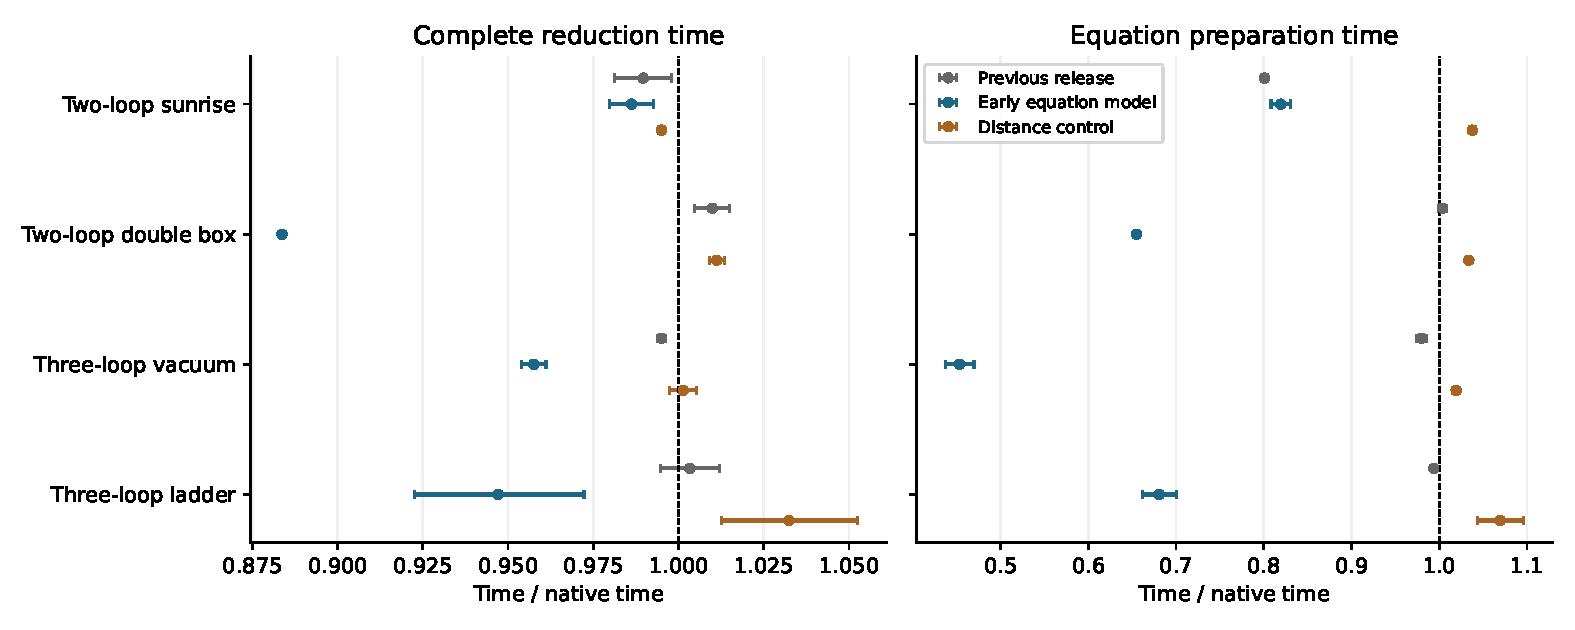
\includegraphics[width=\textwidth]{figures/early_equation_costs.pdf}
 \caption{Complete and equation-preparation time relative to native choices.
 Points use physical-profile weighting and intervals resample profiles.
 Each topology has two new physical profiles.}
 \label{fig:early-equation-costs}
\end{figure}
\begin{figure}[htbp]
 \centering
 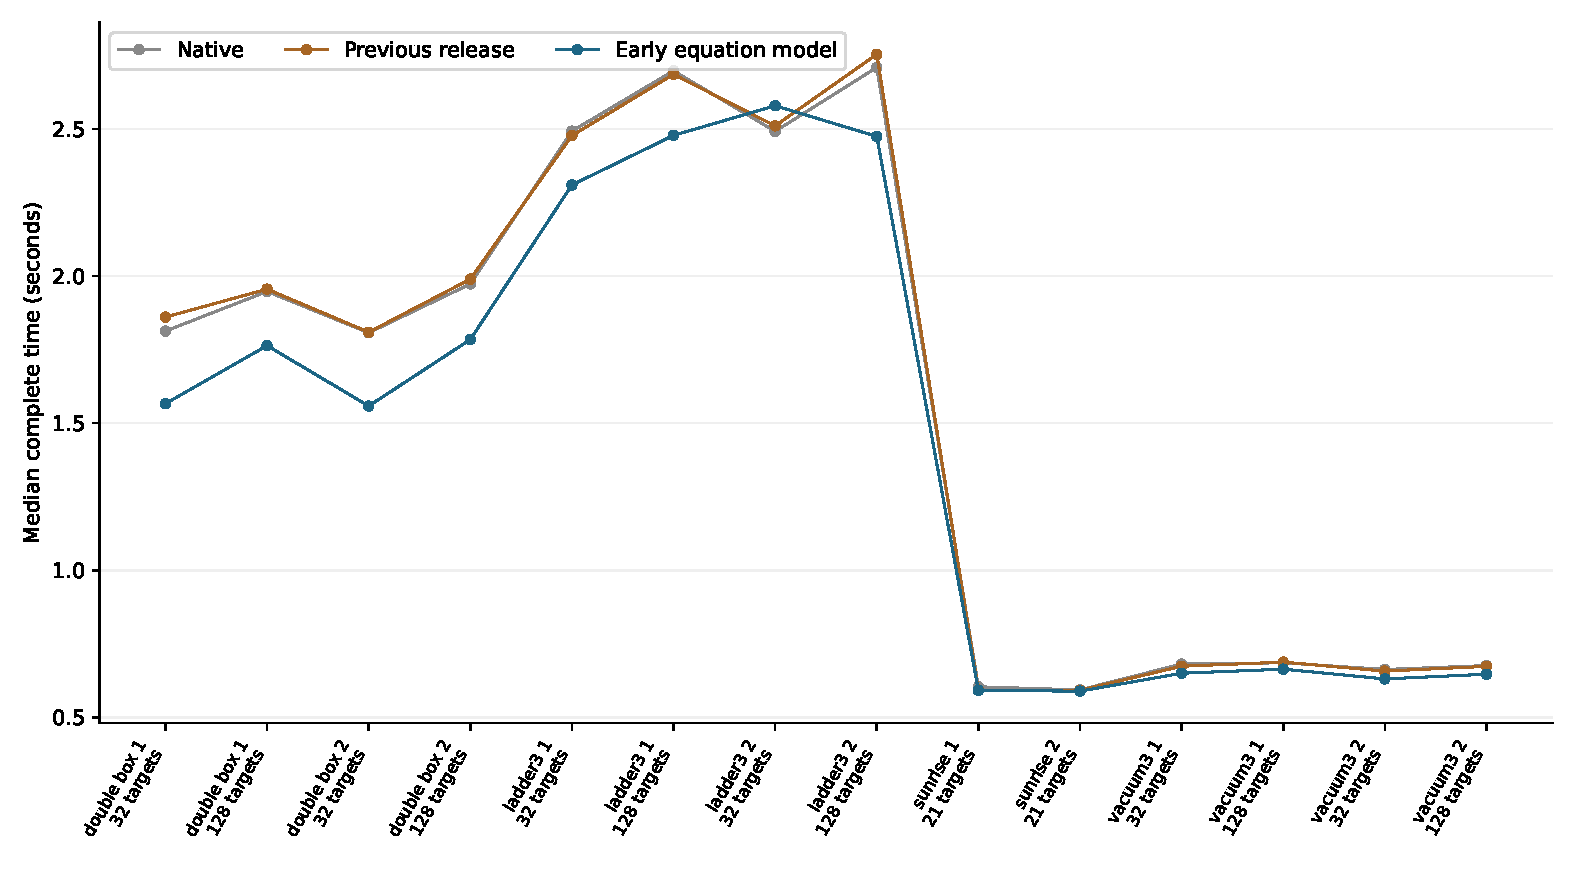
\includegraphics[width=\textwidth]{figures/early_equation_batches.pdf}
 \caption{Median complete time for each fixed target batch, including
 inference, exact checks and all fallback attempts. Each point is the
 median of five alternating repetitions.}
 \label{fig:early-equation-batches}
\end{figure}

All 280 comparison workflows and 8 additional applications pass the independent exact audit. The applications receive only the prescribed basis, and their coefficients agree with the reference after execution. The audit checks 94,970 coefficient pairs, including 1,915 distinct pairs. Every method completes on its first attempt. Maximum sampled memory for Kira and its child processes is 53.46 MiB, and maximum temporary solver storage is 1.39 MiB.

These results test a trained decision before native equation construction,
with complete costs and exact output checks. They establish the measured
domain at fixed rational kinematics. General symbolic multiscale
coefficients, new graph structures, broader target lists and high-loop
reductions require separate evidence. Section~\ref{sec:generalization} supplies subsequent tests on new scattering
structures with independent symbolic invariants. The earlier negative comparisons
remain part of the study, and the selected route activates only the
combinations supported by validation~\cite{KiraEarlyEquationData}.
\FloatBarrier
